\documentclass[10pt,twocolumn]{article}

\usepackage{times}
\usepackage{spverbatim}
\usepackage[swedish]{babel}
\usepackage[utf8]{inputenc}
\usepackage{listings}
\usepackage[toc,page]{appendix}
\usepackage{graphicx}
\usepackage{mathtools}
\usepackage{float}
\usepackage{algorithm}
\usepackage{algpseudocode}
\usepackage[margin={2.45cm, 2.45cm}]{geometry}
\renewcommand\appendixname{Bilagor}
\renewcommand\appendixpagename{Bilagor}
\usepackage[compact]{titlesec}
\titlespacing{\section}{0pt}{*2}{*2}
\raggedbottom
\sloppy

\title{Lab 2\\ \emph{Pthread}}

\author{Martin Söderén \\ marso329, 9009291098 }

\date{\today}

\begin{document}

\maketitle

\clearpage

\section{Introduction}

The problem consists of implementing and parallelizing two image filters using Pthreads. The first filter is a blurfilter that for each pixel calculates a average colour for the surrounding pixels. The other is a threshold filter that calculates the average intensity of the whole picture and makes all pixels above the average black and those below white.

\section{Method}
\subsection{Blur filter algorithm}
No synchronization is needed here because all threads write to a new destination array.
\begin{algorithm}[H]
\caption{Master thread blur filter}
\label{alg:Master}
\begin{algorithmic}
\Procedure{Master}{}
\State Read file
\State Calculate part of image to do
\For{all slave threads}
\State Calculate slave threads part to work on
\State Create new thread using pthread\_create
\EndFor
\State Calculate part of the image
\For{all slave threads}
\State Join thread using pthread\_join
\EndFor
\State Write destination to file
\EndProcedure
\end{algorithmic}
\end{algorithm}

\begin{algorithm}[H]
\caption{Slave thread blur filter}
\label{alg:Slave}
\begin{algorithmic}
\Procedure{Slave}{}
\State Calculate part of the image
\EndProcedure
\end{algorithmic}
\end{algorithm}
\subsection{Threshold filter algorithm}

\begin{algorithm}[H]
\caption{Master thread threshold filter}
\label{alg:Master}
\begin{algorithmic}
\Procedure{Master}{}
\State Read file
\State Calculate which part of the image to work on

\For{all slave threads}
\State Calculate slave threads part to work on
\State Create new thread using pthread\_create
\EndFor

\State Calculate threshold for part of image
\State Add threshold to Mutex protected variable
\State Wait for all threads to call pthread\_barrier\_wait
\State Create part of image
\For{all slave threads}
\State Join thread using pthread\_join
\EndFor
\State Write destination to file
\EndProcedure
\end{algorithmic}
\end{algorithm}

\begin{algorithm}[H]
\caption{Slave thread threshold filter}
\label{alg:Slave}
\begin{algorithmic}
\Procedure{Slave}{}
\State Calculate threshold for part of image
\State Add threshold to Mutex protected variable
\State Wait for all threads to call pthread\_barrier\_wait
\State Create part of image
\EndProcedure
\end{algorithmic}
\end{algorithm}

\subsection{Design}
The image is split up by rows to utilize the space locality of the data and the data in both cases are accessed row wise for improved spatial locality. For example in the blur filter the pixelvalue is not calculated for each radius but for each row. If it was calculated for each radius that meant that we jump in the memory and the probability for cache misses is greater.


\section{Result}
The blur filter scales rather well and hits the lower time limit at around 13 cores with an improvement compared to a single core of 14 times faster. After 13 cores the calculation time remains the same. At that times the cost of starting a new thread is probably equal to the gain from that new thread.
\\
\\
The threshold filter scales somewhat. It levels out at around 7 cores and after that it starts to increase. The calculation time with 7 cores is 3 times better than with a single core. The times are however very short in both cases. The reason for the increase of calculation time with more cores is probably because of the mutex protected threshold variable which every core needs to access to write the local threshold.  
\begin{figure}[H]
	\begin{center}
		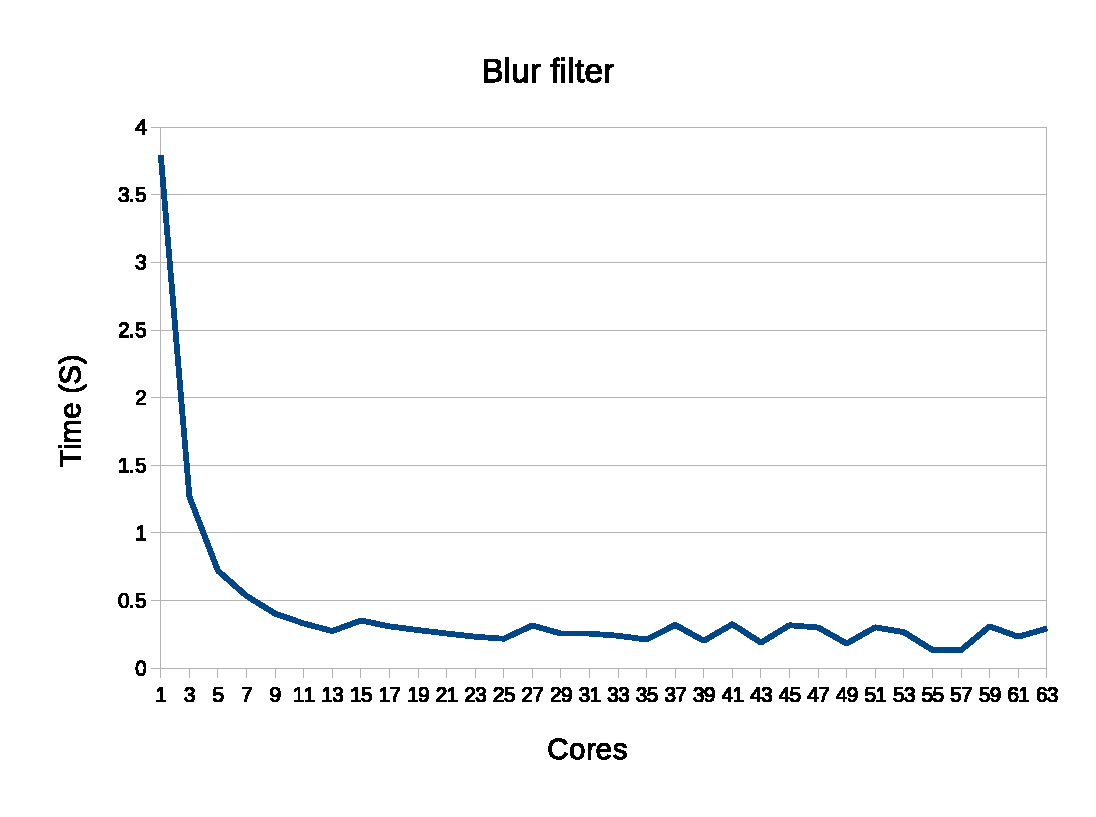
\includegraphics[scale=0.5]{figurer/blur.eps}
	\end{center}
	\caption{Times for blur filter with radius 21}
\end{figure}

\section{Result}
\begin{figure}[H]
	\begin{center}
		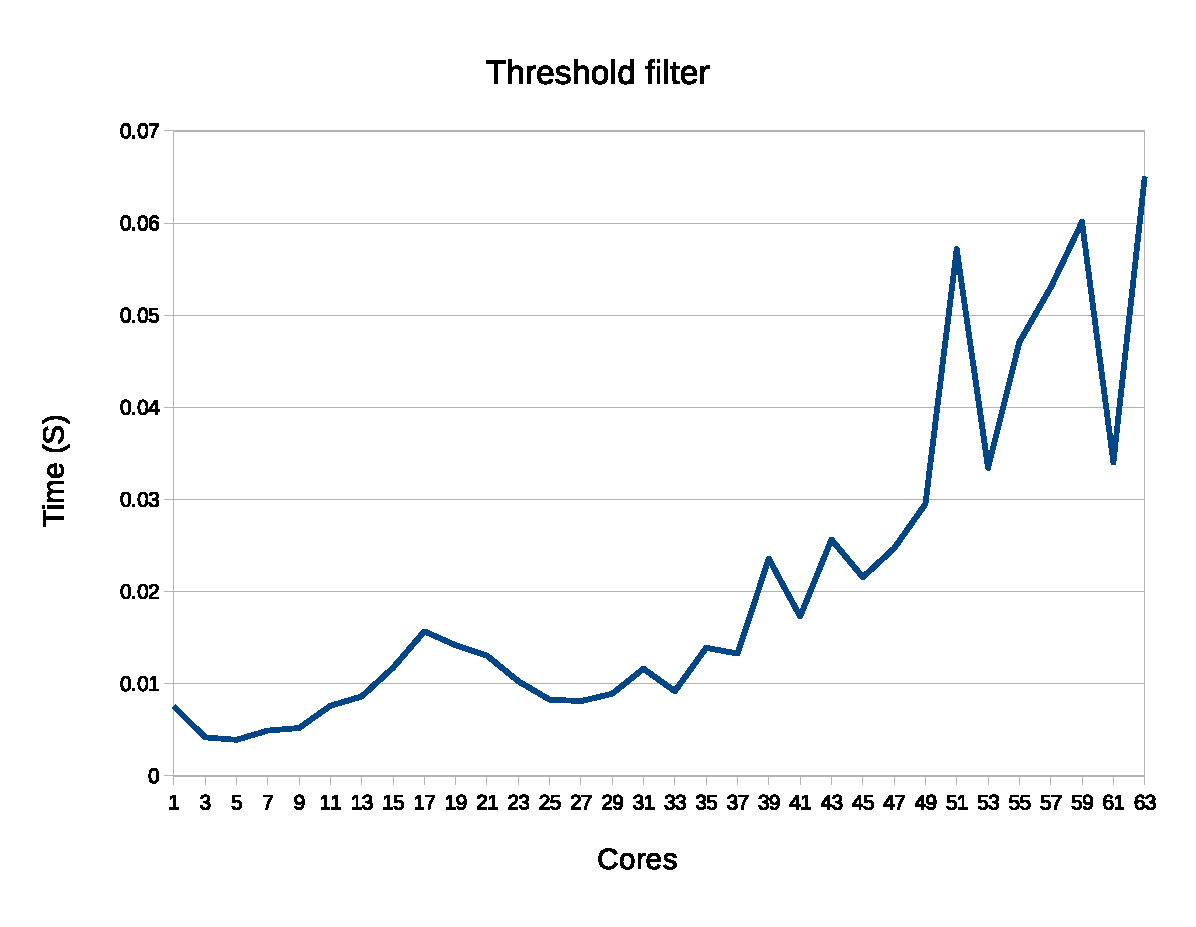
\includegraphics[scale=0.5]{figurer/thres.eps}
	\end{center}
	\caption{Times for threshold filter}
\end{figure}

\newpage

\onecolumn
\appendix
\section{blurthread.c} \label{app:blur}
\lstinputlisting[language=c]{../blurthread.c}

\section{thresthread.c} \label{app:blur}
\lstinputlisting[language=c]{../thresthread.c}

\end{document}
